\documentclass{article}
\usepackage{amsmath}
\usepackage{amssymb}
\usepackage{graphicx}
\usepackage{listings}
\usepackage{xcolor}
\usepackage{geometry}
\usepackage{longtable}
\geometry{a4paper, margin=0.2in}

\title{Dokumentacja Projektowa: System Zarządzania Biblioteką}
\author{Nel Skowronek, Jan Ryszkiewicz}
\date{\today}

\begin{document}

\maketitle

\section{Cel aplikacji}
Celem aplikacji jest stworzenie systemu zarządzania biblioteką umożliwiającego sprawne zarządzanie zasobami książkowymi, autorami, użytkownikami, kategoriami oraz ocenami. System pozwala na przechowywanie informacji o książkach, zarządzanie wypożyczeniami oraz ocenianie książek przez użytkowników.

\section*{Charakterystyka użytkowników}
\begin{itemize}
    \item \textbf{Administrator} – posiada pełne uprawnienia do zarządzania użytkownikami (dodawanie, edycja, usuwanie), a także pełny dostęp do wszystkich funkcjonalności systemu.
    \item \textbf{Bibliotekarz} – posiada uprawnienia do zarządzania książkami, autorami, kategoriami, wypożyczeniami i ocenami, ale nie może zarządzać użytkownikami.
\end{itemize}

\section*{Wymagania funkcjonalne}
\subsection*{Administrator}
\begin{itemize}
    \item Dodawanie, edycja i usuwanie użytkowników.
    \item Zarządzanie książkami, autorami, kategoriami, wypożyczeniami i ocenami.
\end{itemize}

\subsection*{Bibliotekarz}
\begin{itemize}
    \item Dodawanie, edycja i usuwanie książek, autorów, kategorii.
    \item Zarządzanie wypożyczeniami i ocenami.
\end{itemize}

\section*{Model danych}
\subsection*{Encje i relacje}
\begin{itemize}
    \item \textbf{Users} (id, username, password\_hash, email, role, created\_at, updated\_at)
    \item \textbf{Authors} (id, name, birth\_date, biography)
    \item \textbf{Books} (id, title, author\_id, published\_date, isbn, available\_copies)
    \item \textbf{Borrowings} (id, user\_id, book\_id, borrowed\_at, due\_date, returned\_at)
    \item \textbf{Categories} (id, name, description)
    \item \textbf{Ratings} (id, user\_id, book\_id, rating, review, created\_at)
\end{itemize}

\subsection*{Diagram ER}
\begin{center}
    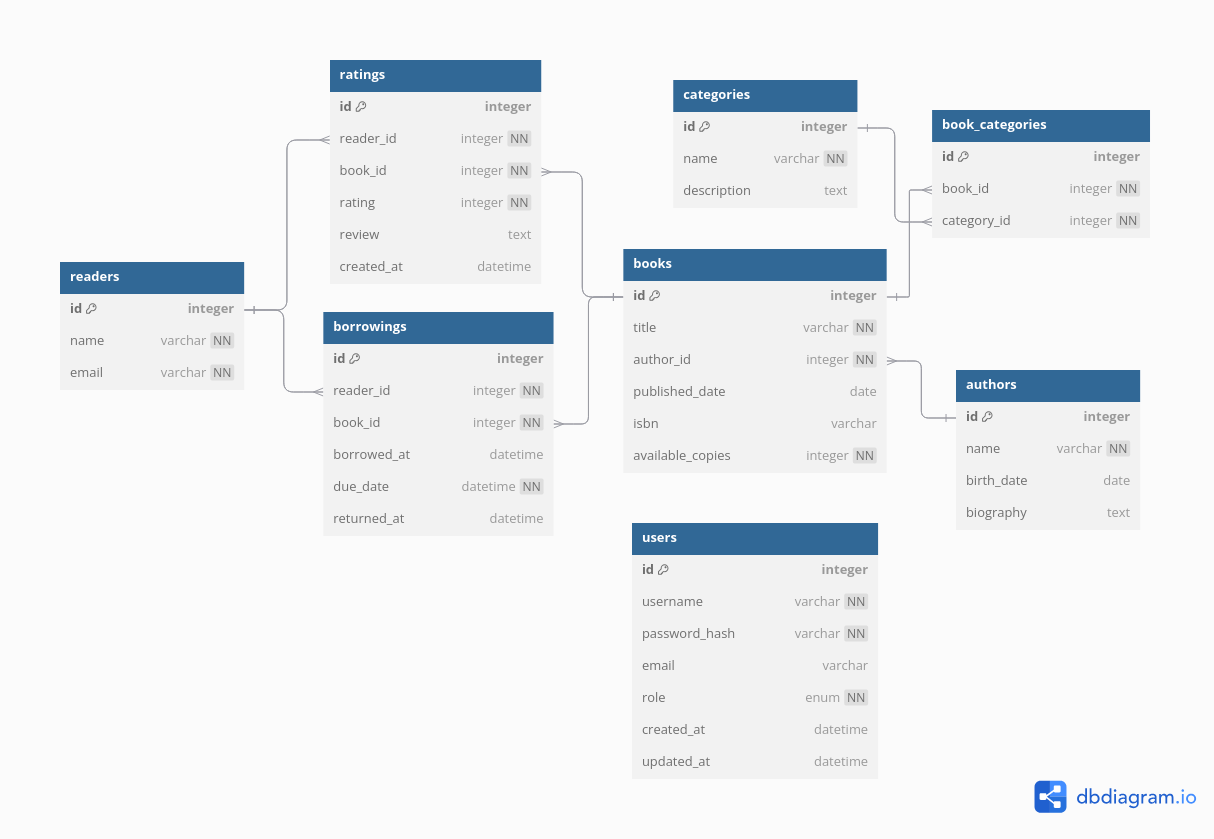
\includegraphics[width=0.8\textwidth]{diagram.png}
\end{center}

\section*{Normalizacja bazy danych}
Wszystkie tabele zostały znormalizowane do 3NF, co zapewnia brak redundancji i spójność danych. Klucze obce definiują relacje między tabelami, co minimalizuje duplikację danych.

\section*{Klucze}
\subsection*{Users}
\begin{itemize}
    \item Klucz główny: \texttt{id}
    \item Klucze kandydackie: \texttt{username}, \texttt{email}
\end{itemize}

\subsection*{Authors}
\begin{itemize}
    \item Klucz główny: \texttt{id}
    \item Klucz kandydacki: \texttt{name}
\end{itemize}

\subsection*{Books}
\begin{itemize}
    \item Klucz główny: \texttt{id}
    \item Klucz kandydacki: \texttt{isbn}
    \item Klucz obcy: \texttt{author\_id} \(\rightarrow\) \texttt{authors(id)}
\end{itemize}

\subsection*{Borrowings}
\begin{itemize}
    \item Klucz główny: \texttt{id}
    \item Klucze obce: \texttt{user\_id} \(\rightarrow\) \texttt{users(id)}, \texttt{book\_id} \(\rightarrow\) \texttt{books(id)}
\end{itemize}

\subsection*{Categories}
\begin{itemize}
    \item Klucz główny: \texttt{id}
    \item Klucz kandydacki: \texttt{name}
\end{itemize}

\subsection*{Ratings}
\begin{itemize}
    \item Klucz główny: \texttt{id}
    \item Klucze obce: \texttt{user\_id} \(\rightarrow\) \texttt{users(id)}, \texttt{book\_id} \(\rightarrow\) \texttt{books(id)}
\end{itemize}

\section*{Prawa dostępu}
\begin{longtable}{|l|p{10cm}|}
\hline
\textbf{Rola} & \textbf{Uprawnienia} \\
\hline
Administrator & Pełny dostęp do zarządzania użytkownikami, książkami, autorami, kategoriami, wypożyczeniami i ocenami. \\
\hline
Bibliotekarz & Zarządzanie książkami, autorami, kategoriami, wypożyczeniami i ocenami. Brak dostępu do zarządzania użytkownikami. \\
\hline
\end{longtable}


\end{document}

